\documentclass[11pt]{article}\usepackage[]{graphicx}\usepackage[]{color}
% maxwidth is the original width if it is less than linewidth
% otherwise use linewidth (to make sure the graphics do not exceed the margin)
\makeatletter
\def\maxwidth{ %
  \ifdim\Gin@nat@width>\linewidth
    \linewidth
  \else
    \Gin@nat@width
  \fi
}
\makeatother

\definecolor{fgcolor}{rgb}{0.345, 0.345, 0.345}
\newcommand{\hlnum}[1]{\textcolor[rgb]{0.686,0.059,0.569}{#1}}%
\newcommand{\hlstr}[1]{\textcolor[rgb]{0.192,0.494,0.8}{#1}}%
\newcommand{\hlcom}[1]{\textcolor[rgb]{0.678,0.584,0.686}{\textit{#1}}}%
\newcommand{\hlopt}[1]{\textcolor[rgb]{0,0,0}{#1}}%
\newcommand{\hlstd}[1]{\textcolor[rgb]{0.345,0.345,0.345}{#1}}%
\newcommand{\hlkwa}[1]{\textcolor[rgb]{0.161,0.373,0.58}{\textbf{#1}}}%
\newcommand{\hlkwb}[1]{\textcolor[rgb]{0.69,0.353,0.396}{#1}}%
\newcommand{\hlkwc}[1]{\textcolor[rgb]{0.333,0.667,0.333}{#1}}%
\newcommand{\hlkwd}[1]{\textcolor[rgb]{0.737,0.353,0.396}{\textbf{#1}}}%
\let\hlipl\hlkwb

\usepackage{framed}
\makeatletter
\newenvironment{kframe}{%
 \def\at@end@of@kframe{}%
 \ifinner\ifhmode%
  \def\at@end@of@kframe{\end{minipage}}%
  \begin{minipage}{\columnwidth}%
 \fi\fi%
 \def\FrameCommand##1{\hskip\@totalleftmargin \hskip-\fboxsep
 \colorbox{shadecolor}{##1}\hskip-\fboxsep
     % There is no \\@totalrightmargin, so:
     \hskip-\linewidth \hskip-\@totalleftmargin \hskip\columnwidth}%
 \MakeFramed {\advance\hsize-\width
   \@totalleftmargin\z@ \linewidth\hsize
   \@setminipage}}%
 {\par\unskip\endMakeFramed%
 \at@end@of@kframe}
\makeatother

\definecolor{shadecolor}{rgb}{.97, .97, .97}
\definecolor{messagecolor}{rgb}{0, 0, 0}
\definecolor{warningcolor}{rgb}{1, 0, 1}
\definecolor{errorcolor}{rgb}{1, 0, 0}
\newenvironment{knitrout}{}{} % an empty environment to be redefined in TeX

\usepackage{alltt}
\renewcommand{\baselinestretch}{1.8}

\usepackage[sort&compress]{natbib}
%\bibliographystyle{..//refs/styles/newphyto.bst}

\usepackage{textcomp}
\usepackage{fontenc}
\usepackage{graphicx}
\usepackage{caption} % for Fig. captions
\usepackage{gensymb} % for \degree
\usepackage{placeins} % for \images
\usepackage[margin=1in]{geometry} % to set margins
\usepackage{setspace}
\usepackage{lineno}
\usepackage{float}
%\usepackage{cite}
\usepackage{amssymb} % for math symbols
\usepackage{amsmath} % for aligning equations
\renewcommand{\thetable}{S\arabic{table}}
\renewcommand{\thefigure}{S\arabic{figure}}
\linenumbers
\usepackage{xr-hyper}
\externaldocument{reconcilingFLS_main_wbbl}

\def\labelitemi{--}
\parindent=24pt
\title{\textit{New Phytologist} Supporting Information}
\date{}
\IfFileExists{upquote.sty}{\usepackage{upquote}}{}
\begin{document}
\maketitle

\noindent \textbf{Article title:} Reconciling competing hypotheses regarding flower-leaf sequences in temperate forests for fundamental and global change biology\\
\noindent \textbf{Authors:} D.M. Buonaiuto, I. Morales-Castilla, E.M. Wolkovich\\

\noindent The following Supporting Information is available for this article:\\


\section*{Figures}


\begin{figure}[H]
    \centering
 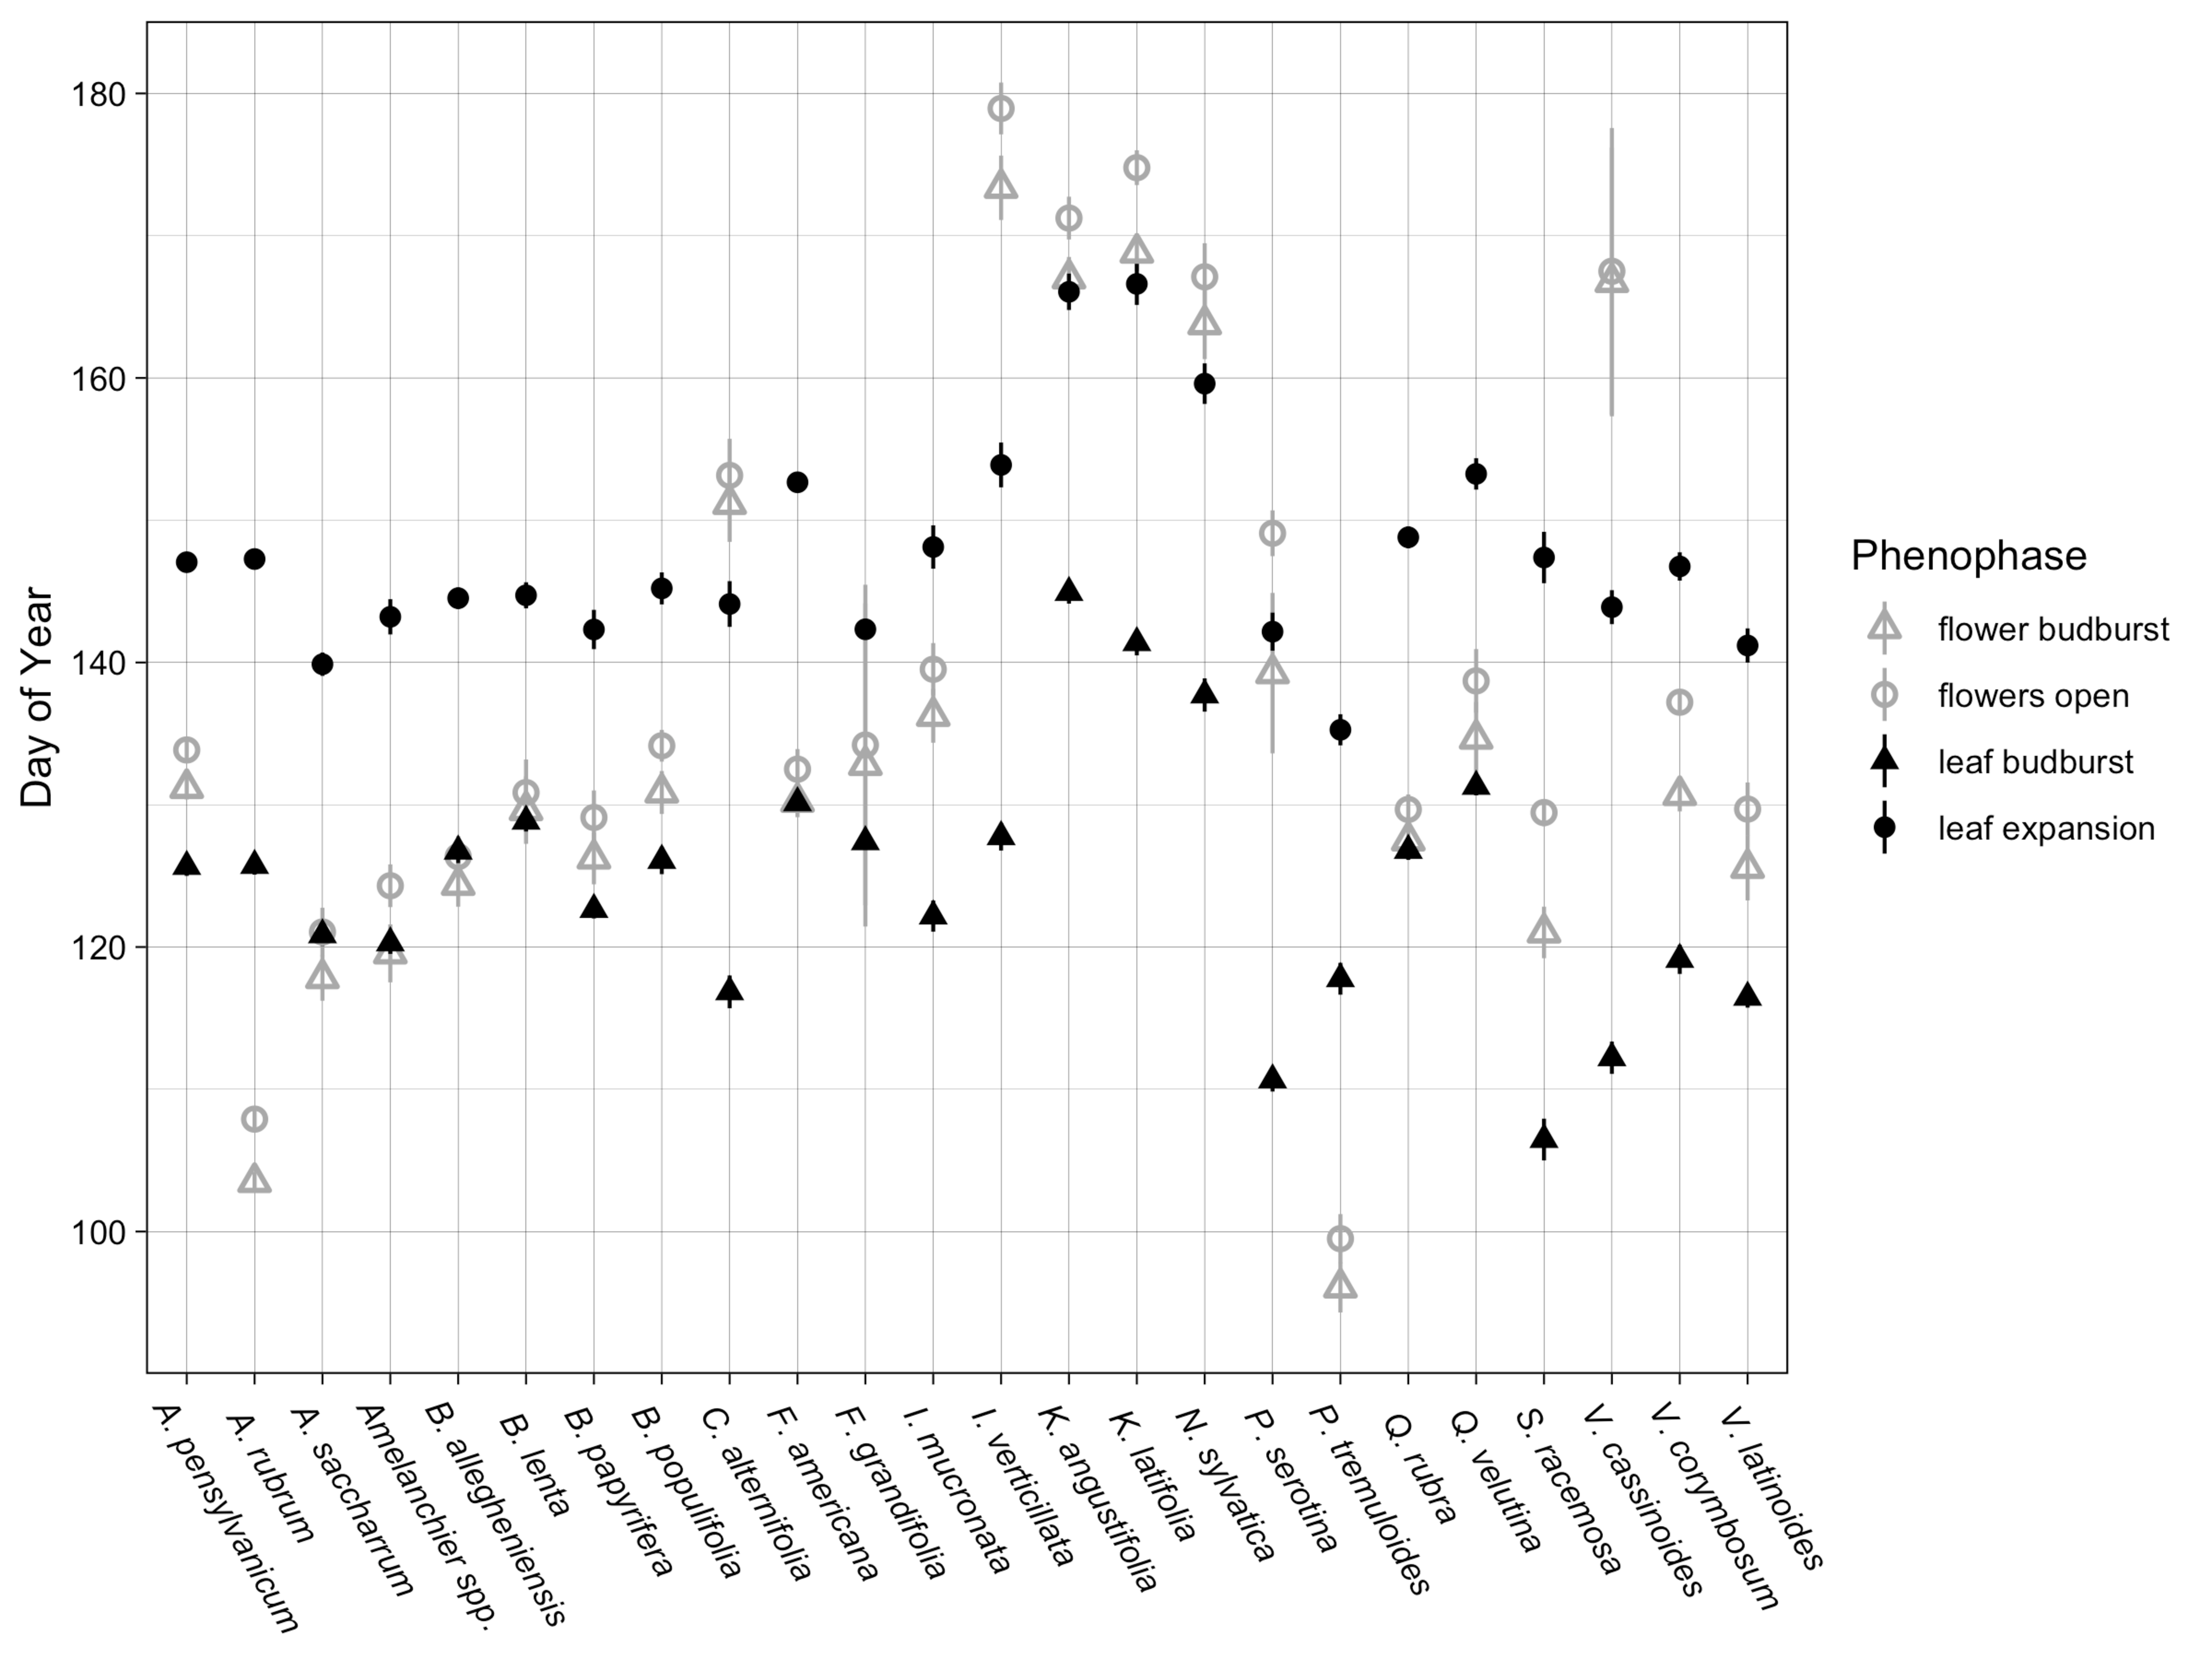
\includegraphics[width=\textwidth]{figure/FigS1.tiff} 
    \caption{\textbf{Quantitative FLS patterns for woody plants at Harvard Forest in Pertersham, MA.} Because phenological sequences consist of several sub-stages if is difficult to unambiguously categorize many species into the current FLS categories. }
    \label{fig:HFmeans}
\end{figure}

\begin{figure}[H]
    \centering
 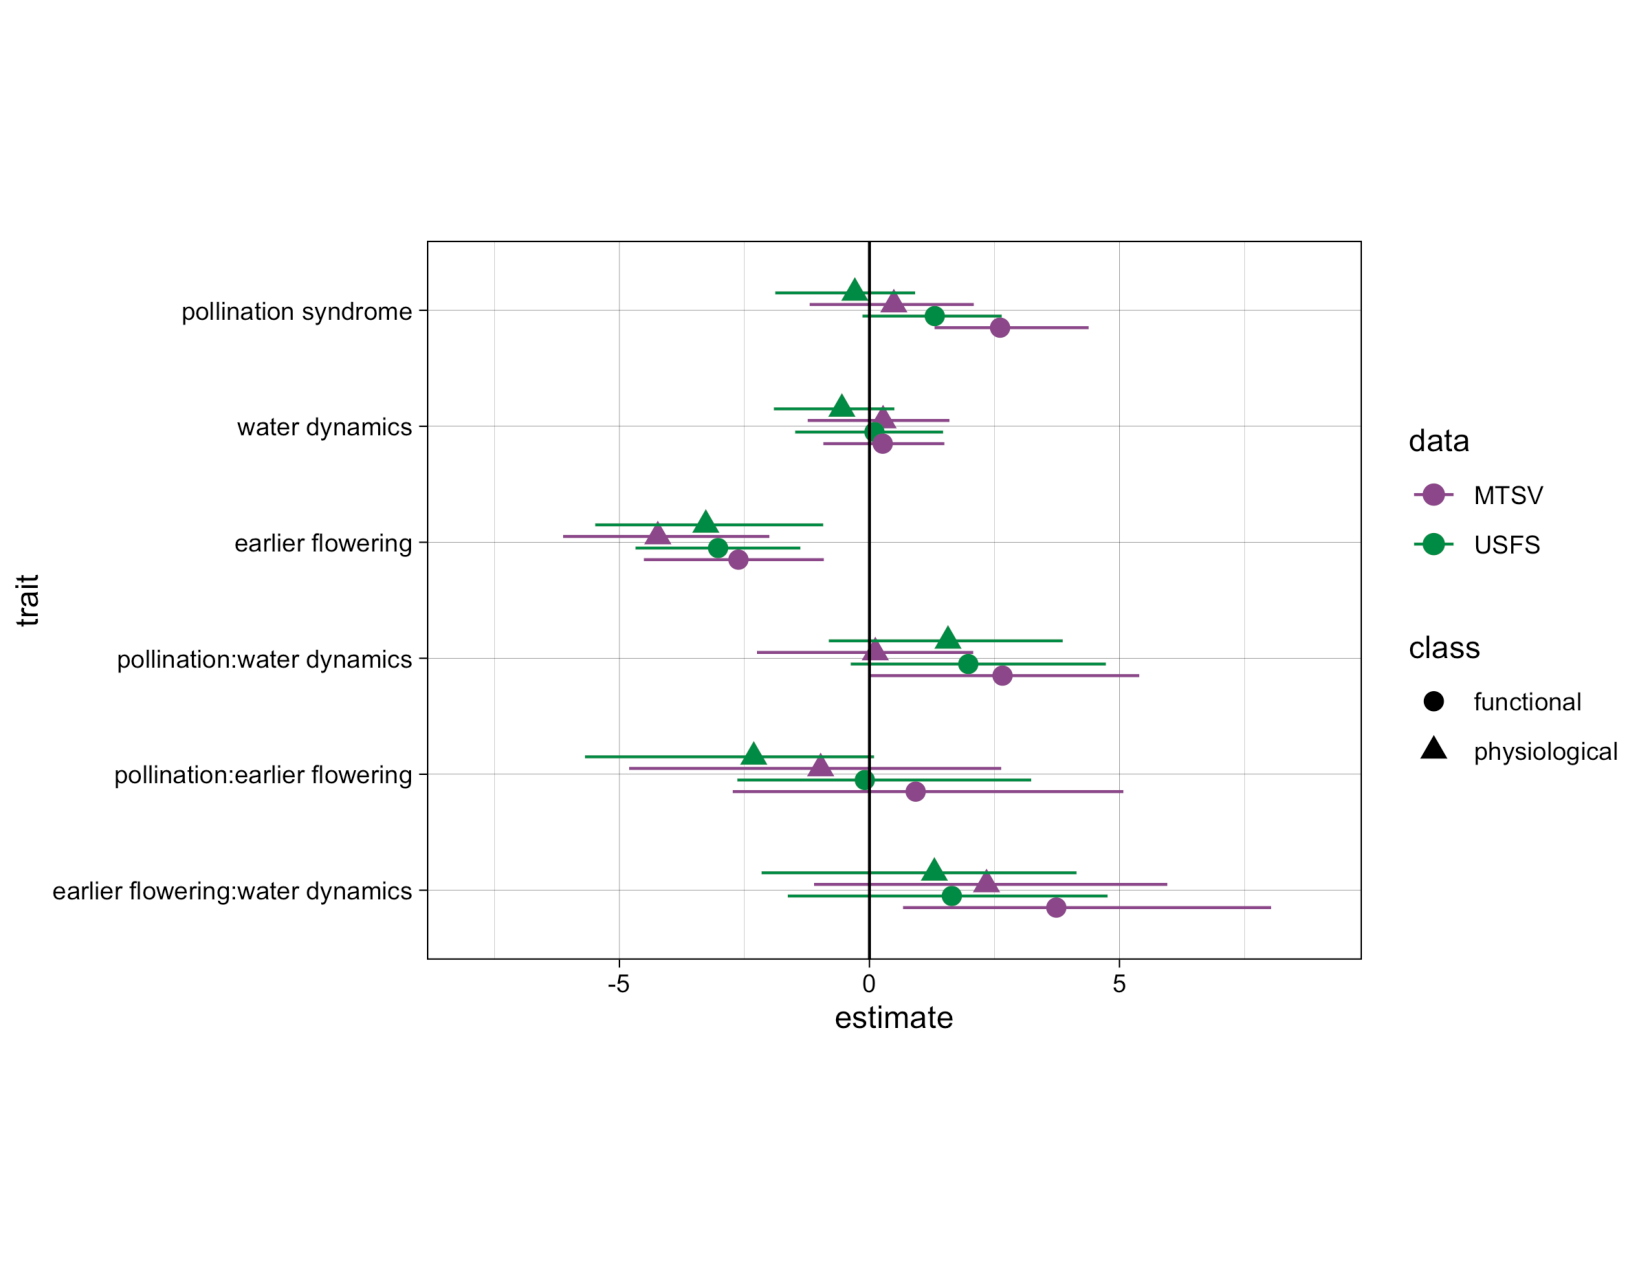
\includegraphics[width=\textwidth]{figure/FigS2.tiff} 
    \caption{\textbf{Mean estimates of the effects of FLS predictors on the likelihood a species is hysteranthous vary across datasets and definitions of FLS.}  We used phylogenetic adjustments and standardized units to make a basic comparison of two datasets (Michigan Trees, Michigan Shrubs and Vines (MTSV) \citep{Barnes2004,Barnes2016} and The United States Silvics Manual (USFS) \citep{Burns1990}) and classes (physiological= no overlap between flowering and leafing, functional= moderate overlap) of FLS. While there is some agreement across models (strong effects of flowering time, no consistent effect interactions between predictors), the effect of other predictors (pollination syndrome, water dynamics) were highly sensitive to how data were defined, potentially biasing any inference from models and compromising the ability to validate the existing FLS hypotheses. Lines represent 95\% bootstrap intervals.}
    \label{fig:muplots.USMT}
\end{figure}

\begin{figure}[H]
\centering
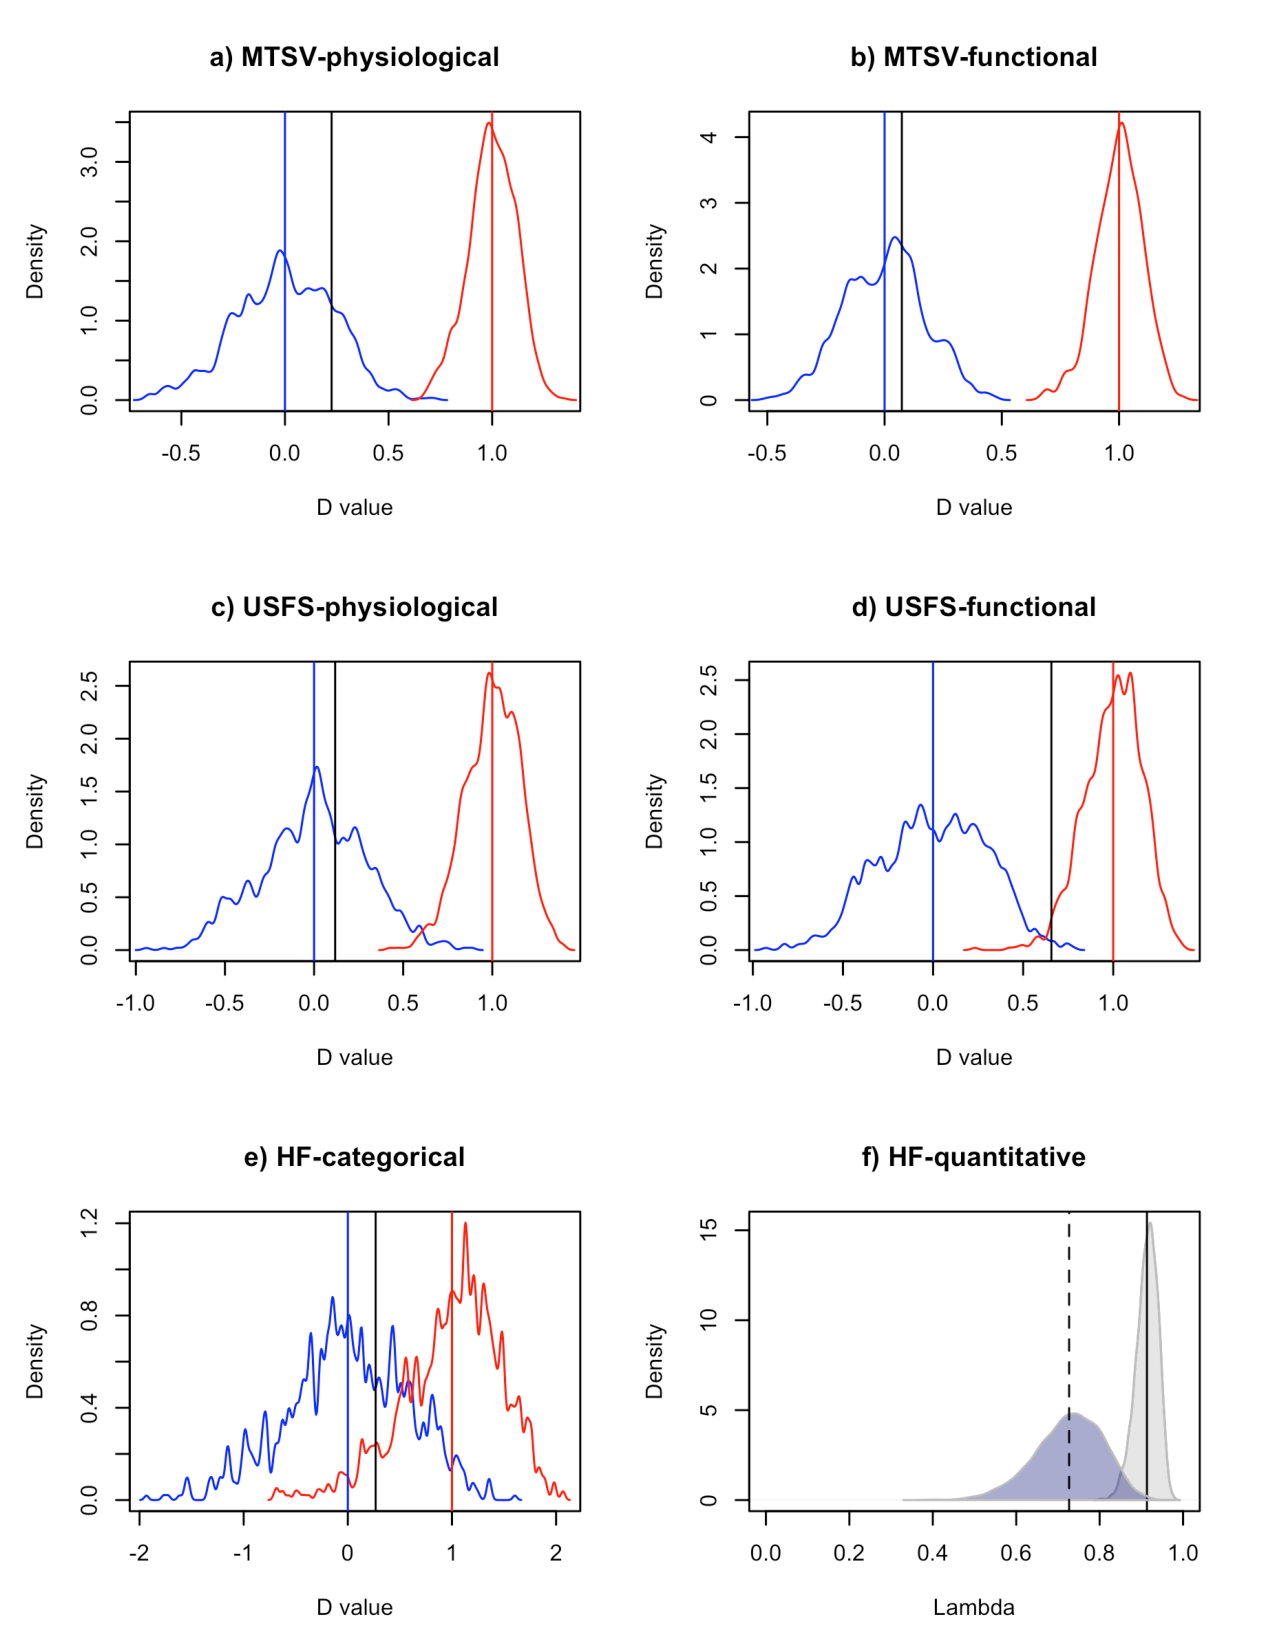
\includegraphics[height=0.9\textheight]{figure/FigS3.tiff} 
  \caption{\textbf{The phylogenetic signal for FLS varies between datasets, and is sensitive to how FLS patterns are categorized.} In a)-e),the black vertical line show the the Fritz's D statistic for binary classifications of FLS estimated from the data, with blue and red lines representing expected D values based on simulations under Brownian threshold model and random model respectively. Panel f) shows the the estimated $\lambda$ values of FLS from the the continuous modeling framework. The solid line indicates the mean estimate of $\lambda$ in the intercept only model and the dashed line indicates the mean estimate of $\lambda$ when all predictors were included in the model. Higher values indicate stronger phylogenetic structure.}
    \label{fig:Dstat}
    \end{figure}

\begin{figure}[H]
\centering
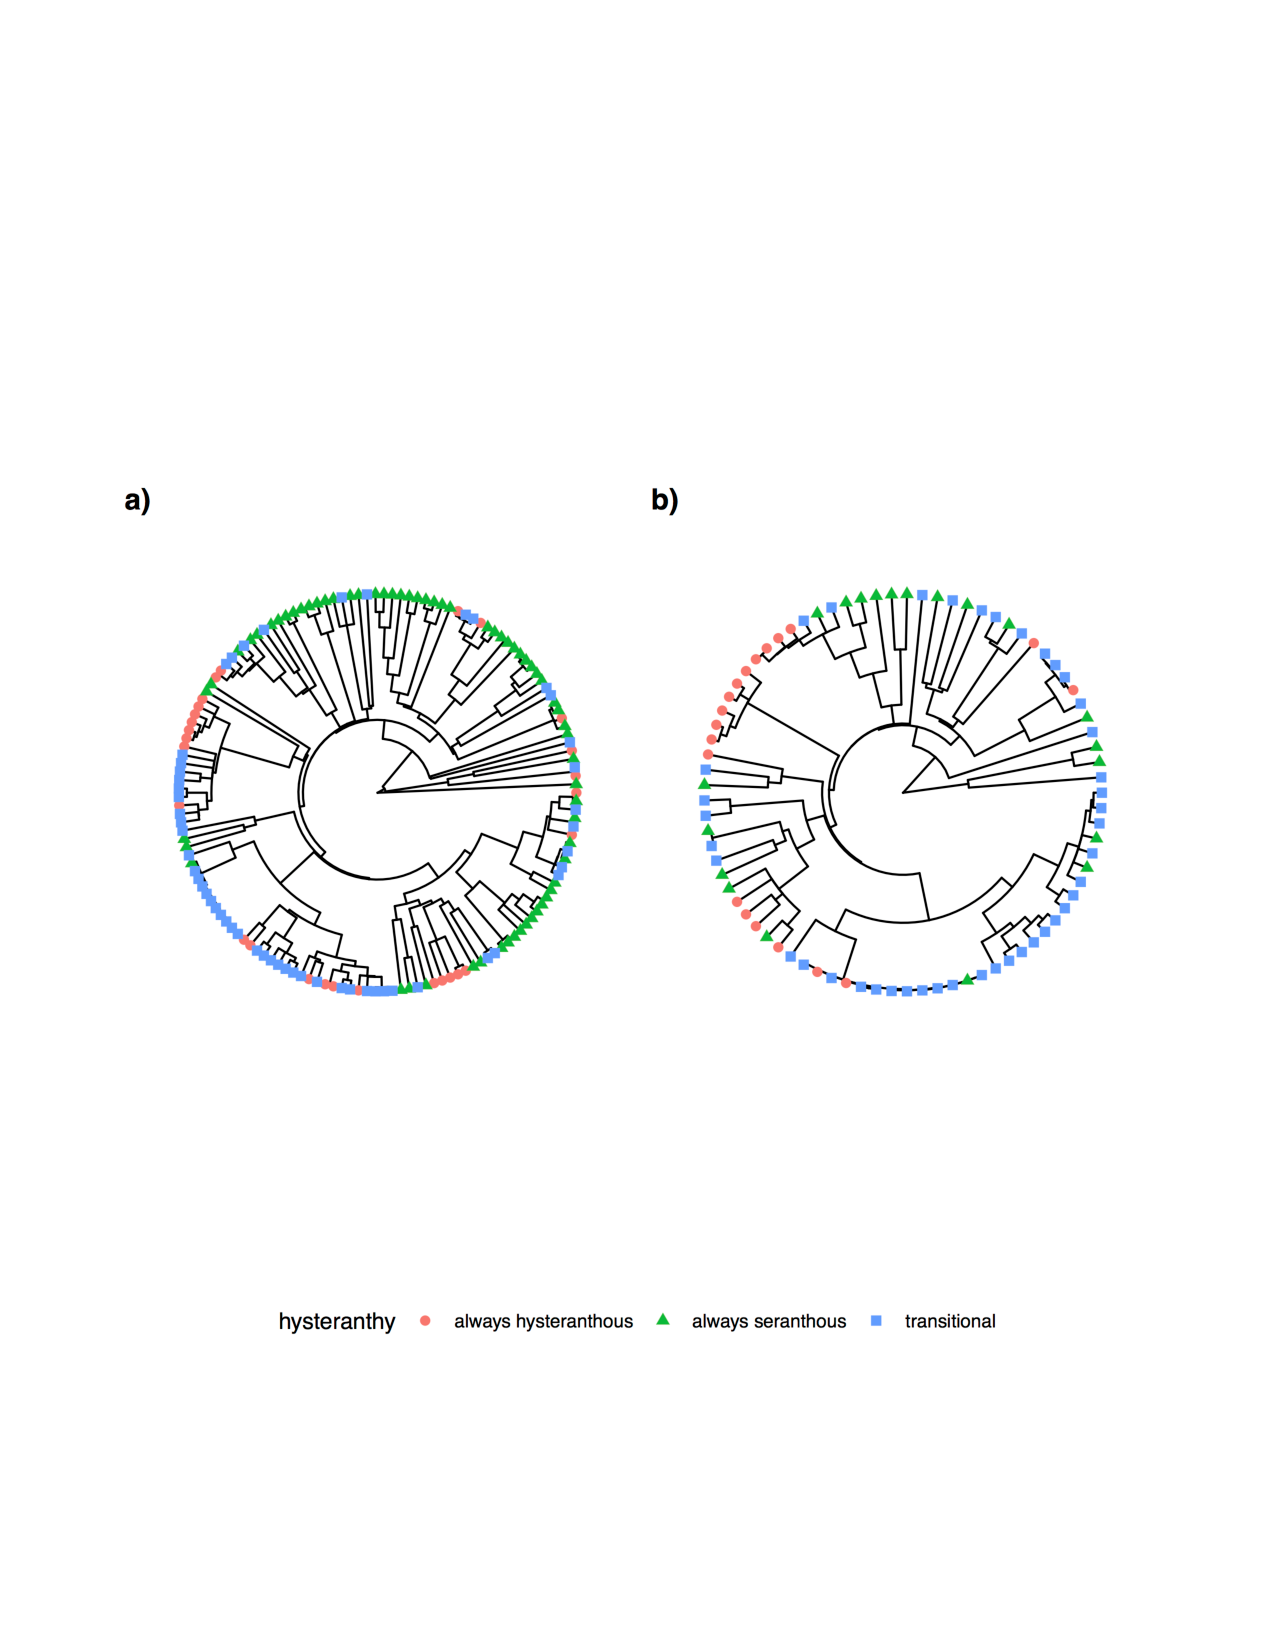
\includegraphics[height=0.9\textheight]{figure/FigS4.tiff} 
  \caption{\textbf{Phylogenetic structure of FLS in MTSV \textbf{a)} and USFS \textbf{b)} varies significantly depending on how FLSs are defined.} Many species are re-assigned to either hysteranthy or seranthy depending on whether FLS is defined functionally (partial overlap between flowering and leafing allowed) or physiologically (no overlap between flowering and leafing allowed) (blue squares). This modeling choice dramatically alters FLS patterning across the tree, resulting in an unstable phylogenetic signal for this trait.}
    \label{fig:phylogeny}
    \end{figure}

\pagebreak[4]


\section*{\nameref{Methods S1}}\label{Methods S1}

\subsubsection*{Climate Change and FLS:}
To evaluate how FLS patterns have changed over time in association with climate change we obtained phenological data for four European woody plant species with long term phenology records of both flower (BBCH 60) and leafout phenology (BBCH 11) from the Pan European Phenological Database \citep{PEP725}. We restricted the data set to include only stations with more than 50 years of data. Following conventions for modeling effects of climate change, we modeled the number of days between flowering and leafing as a function of time for each species, using a hinge model with 1980 as a break point \citep{IPCC2013,Kharouba2018}. For each species, we display the pre-1980 mean and 95\% credible intervals of the time between flowering and leafing and the post-1980 change in mean time between phenophases that can be  attributed to climate change (Fig. \ref{fig:climchange}).

\subsubsection*{Modeling FLS variation in MTSV and USFS data}
For these two, categorical, species-level case-studies, we converted verbal descriptions of flower-leaf sequences into a binary response variable. For our more inclusive ``functional" definition of hysteranthy, which allows for some overlap between floral and vegetative phenophases, we included species entries with descriptions \textit{``flowers before the leaves"}, \textit{``flowers before or with leaves"} and \textit{``flowers with leaves"} as hysteranthous. Our more restrictive ``physiological" hysteranthy definition only included species described as \textit{``flowers before the leaves"} as hysteranthous.\\

\noindent For modeling trait associations with FLS, we chose three predictors to represent the three major FLS hypotheses; pollination syndrome, average flowering time and minimum precipitation levels across the species range. We obtained pollination syndrome and average flowering time information directly from the respective data sources and estimates of minimum precipitation across range from the USDA/NRCS Conservation Plants Characteristics database \citep{usdancrs}. We coded pollination syndrome as biotic- or wind-pollinated, and assigned known ambophilous species in the genus \textit{Salix} as biotic-pollinated. We re-coded flowering time as the average of the range of months of flowering reported in each data source.\\

\noindent For these case studies, we modeled associations between hysteranthy and the trait predictors with all two-way interactions with logistical regressions in phylogenetic generalized linear modeling framework \citep{Ives2010} using the R package ``phylolm" \citep{Ho2014}. Model results are presented in Fig. \ref{fig:muplots.USMT}. Our models incorporated a published angiosperm phylogenetic tree \citep{Zanne2013} pruned to match the species list for each case study. Species found in the trait data set but not in the original phylogenetic tree were added to the pruned tree at the generic root. In total, 32 species were added to the generic roots for the MTSV data set and eight for the USFS data set. We visualized phylogenetic patterning of FLS across the tree of each case study (Fig. \ref{fig:phylogeny}). The MTSV analysis was based on trait and FLS data for 147 species and the USFS analysis on 81 species. \\

\noindent We ran the models with 599 bootstrapped re-sampling iterations for each data set \citep{Wilcox2010}. We standardized all predictors by subtracting the mean and dividing by two standard deviations to allow for a reasonable comparison of effect sizes between the binary and continuous predictors in this model \citep{Gelman2007}. 


\subsubsection*{Harvard Forest models}
From the publicly available Harvard Forest phenology data \citep{Okeefe2015} we calculated the time between flowers opening and leaves reaching 75\% of their final size for each individual tree per year in the data. Positive FLS values indicate flowering-first and negative values leafing-first. To compare the inference between categorical and continuous measure of FLS, we re-coded the continuous FLS measures as binary responses with positive values coded as hysteranthous and negative values as seranthous. These models used the same predictors as the MTSV and USFS datasets (flowering time, pollination syndrome, minimum precipitation across species' range and all two way interactions between predictors), except that we estimated flowering time directly from the HF data for each individual/year. The Harvard Forest analysis included 23 species. While taxonomically limited compared to the MTSV and USFS data, this data set included repeated phenology observation per species over time, and within year variation between individuals per species. \\ 
For both the categorical and continuous Harvard forest models we used a Bayesian phylogenetic mixed modeling framework (PMM) \citep{Garamszegi2014} using the R package ``brms" \citep{Burkner2018}. PMM's incorporate the phylogenetic relationship among species as a random effect, utilizing a variance-covariance matrix based on species relationships to account for the non-independence in the model residuals that can be explained by phylogeny. We also included species as an additional random effect to account for non-independence in the residuals than is not due to phylogeny, and included individual as a nested factor within this random intercept to account for the repeat observations over time. The categorical model was built on a Bernoulli likelihood distribution and the continuous model on a Gaussian distribution. For both models, we ran 4 chains with 4000 iterations and a warm-up of 3000 iterations each, resulting in 4000 total sampling iterations. All models used weakly informative priors on the intercept and error terms. Increasing priors three-fold did not impact the model estimates. As our primary goal was to directly compare the effects each predictor, we standardized these variables to allow for a reasonable comparison between them {\citep{Gelman2007}. Model results can be found in Fig. \ref{fig:muplots.HF}.\\

%\noindent The three Harvard Forest models are detailed below:\\
%\begin{enumerate}
%\item \underline{Categorical model}:\\
%Pr(y_i &=1) &= logit^{-1} \alpha_{sp[i]} + \alpha_{phylo[i]} + \beta_{pollination syndrome}X_1_[_i_] + \beta_{flowering time}X_2_[_i_] + \beta_{min. precipitation}X_3_[_i_] +\beta_{pollination syndrome}:\beta_{flowering time}X_4_[_i_]+\beta_{pollination syndrome}:\beta_{min. precipitation}X_5_[_i_]+ \beta_{flowering time}:\beta_{min. precipitation}X_6_[_i_] + \epsilon_i\\
%
%\epsilon_i & \sim N(0,\sigma^2_y) \\ 
%
%\noindent The influence of the phylogeny $\alpha_phylo$ was modeled as follows:\\
%\alpha_{sp} & \sim N(\mu_{\alpha}, COR[\sigma^2_{phylo}]) \\
%
%\noindent THe $\alpha$ for species effects indendent of the phylogeny was modeled as follows:\\
%\alpha_{sp} & \sim N(\mu_{\alpha}, \sigma^2_{species}) \\
%
%\item \underline{Continuous model}: \\
%y_i &= \alpha_{ind/sp[i]} +\alpha_{phylo[i]} + \beta_{pollination syndrome}X_1_[_i_] + \beta_{flowering time}X_2_[_i_] + \beta_{min. precipitation}X_3_[_i_] +\beta_{pollination syndrome}:\beta_{flowering time}X_4_[_i_]+\beta_{pollination syndrome}:\beta_{min. precipitation}X_5_[_i_]+ \beta_{flowering time}:\beta_{min. precipitation}X_6_[_i_] + \epsilon_i\\

%\epsilon_i & \sim N(0,\sigma^2_y) \\ %I Think this is wrong and should reflect the phyogeny
%
%
%\noindent The effect of the phylogeny was model as above and here, the individual effects within species were modeled:\\
%\alpha_{ind/sp} & \sim N(\mu_{\alpha}, \sigma^2_{ind/sp}) \\

%\item \underline{Inter-annual model}:\\
%y_i &= \alpha_{i} + \beta_{annual precipitation}X_1[_i_] + \epsilon_i\\
%\epsilon_i & \sim N(0,\sigma^2_y) \\

%\end{enumerate}
\indent We calculated the marginal effects for the Harvard Forest continuous model using the R-package ``ggeffects" \citep{Ludecke2018}. Figure \ref{fig:apcs} shows the water dynamics effect of FLS given a flowering day of May 1 (close to the average flowering date for the whole community overtime). This same relationship between pollination syndrome and minimum precipitation remained evident across flowering dates from mid April-June (see Fig. \ref{fig:apcs}). \\

\noindent Though we make broad comparisons between the HF and MTSV/USFS case studies, differences in data structure between the datasets required us to use alternative modeling frameworks. The MTSV and USFS data provide one response variable for each species while the HF data contains intra-specific differences in FLS, providing several different response values per species. The current phylogenetic generalized linear model framework can only fit models with one response value per species, while the phylogenetic mixed model in brms may over-fit models with this kind of data structure and performs better on multi-response per species datasets like HF \citep{BurknerPC}. We ran both model types on each case study and while they do yield different absolute estimates, the patterns we found were consistent across each framework, and we report results from the most accurate model for each dataset.\\

\subsubsection*{Analyses of phylogenetic signal}
For all categorical specifications of FLS (MTSV, USFS and HF), we assessed the phylogenetic structure of hysteranthous flowering in all  with Fritz's D-statistic \citep{FRITZ2010} using the ``Caper" package \citep{Orme2013} in R. Fritz's D calculates the sum of changes in estimated node values of a binary trait along edges in a phylogeny and compares this observed value to both a model of phylogenetic randomness and Brownian threshold model. The means of the two data simulations scale values of D to set points of 0 (as phylogenetically conserved) and 1 (random)  \citep{Orme2013}. We visualized the distribution of the traits across the tree for the MTSV and USFS datasets using the R package ``ggtree" \citep{Yu2017}, (see Fig. \ref{fig:phylogeny}).\\

\noindent For the quantitative Harvard Forest model, we estimated the phylogenetic signal for FLS (lambda) directly from the PMM model. To estimate lambda, we fit an intercept-only model with the phylogeny covariance matrix as a random effect and obtained the intra-class correlation value which is the phylogenetic signal. We also estimated the phylogenetic signal from the full model which included all predictors, and in both cases the intra-class correlation in the residuals were high. Estimated phylogenetic signals from all case studies are reported in (Fig. \ref{fig:Dstat}).  % I can probabalby elaborate on this. 
  
  
\clearpage

%\bibliography{..//refs/hyst_outline.bib}
\begin{thebibliography}{20}
\expandafter\ifx\csname natexlab\endcsname\relax\def\natexlab#1{#1}\fi

\bibitem[{Barnes \emph{et~al.}(2016)Barnes, Dick \& Gunn}]{Barnes2016}
{\bf Barnes BV, Dick CW, Gunn ME}. 2016.
\newblock \emph{Michgan Shrubs & Vines: A guide to species of the Great Lakes
  Region}.
\newblock University of Michigan Press.

\bibitem[{Barnes \& Wagner(1981,2004)}]{Barnes2004}
{\bf Barnes BV, Wagner WHJ}. 1981,2004.
\newblock \emph{Michigan Trees: A guide to the Trees of the Great Lakes
  Region}.
\newblock University of Michigan Press.

\bibitem[{B{\"u}rkner(2017)}]{BurknerPC}
{\bf B{\"u}rkner PC}. 2017.
\newblock brms-users group.
\newblock personal communication.

\bibitem[{B{\"u}rkner(2018)}]{Burkner2018}
{\bf B{\"u}rkner PC}{\bf . 2018}.
\newblock Advanced bayesian multilevel modeling with the r package brms.
\newblock \emph{R Journal}, {\bf 10}: 395--411.

\bibitem[{Burns \& Honkala(1990)}]{Burns1990}
{\bf Burns RM, Honkala BH}. 1990.
\newblock Silvics of North America: Volume 2. hardwoods.
\newblock Tech. rep., United States Department of Agriculture (USDA), Forest
  Service.

\bibitem[{{Daniel L{\"u}decke}(2018)}]{Ludecke2018}
{\bf {Daniel L{\"u}decke}}{\bf . 2018}.
\newblock ggeffects: Tidy data frames of marginal effects from regression
  models.
\newblock \emph{{Journal of Open Source Software}}, {\bf 3}: 772.

\bibitem[{Fritz \& Purvis(2010)}]{FRITZ2010}
{\bf Fritz SA, Purvis A}{\bf . 2010}.
\newblock Selectivity in mammalian extinction risk and threat types: a new
  measure of phylogenetic signal strength in binary traits.
\newblock {\bf 24}: 1042--1051.

\bibitem[{Gellman \& Hill(2997)}]{Gelman2007}
{\bf Gellman A, Hill J}. 2997.
\newblock \emph{Data analysis using regression and multilevel/hierarchical
  models}.
\newblock Cambridge University Press.

\bibitem[{Ho \& Ane(2014)}]{Ho2014}
{\bf Ho LST, Ane C}{\bf . 2014}.
\newblock A linear-time algorithm for gaussian and non-gaussian trait evolution
  models.
\newblock \emph{Systematic Biology}, {\bf 63}: 397--408.

\bibitem[{Ives \& Garland(2010)}]{Ives2010}
{\bf Ives AR, Garland Jr. T}{\bf . 2010}.
\newblock Phylogenetic logistic regression for binary dependent variables.
\newblock \emph{Systematic Biology}, {\bf 59}: 9--26.

\bibitem[{Kharouba \emph{et~al.}(2018)Kharouba, Ehrl{\'e}n, Gelman, Bolmgren,
  Allen, Travers \& Wolkovich}]{Kharouba2018}
{\bf Kharouba HM, Ehrl{\'e}n J, Gelman A, Bolmgren K, Allen JM, Travers SE,
  Wolkovich EM}{\bf . 2018}.
\newblock Global shifts in the phenological synchrony of species interactions
  over recent decades.
\newblock \emph{Proceedings of the National Academy of Sciences}, {\bf 115}:
  5211.

\bibitem[{O'Keefe(2015)}]{Okeefe2015}
{\bf O'Keefe J}. 2015.
\newblock Phenology of woody species at Harvard Forest since 1990.

\bibitem[{Orme \emph{et~al.}(2013)Orme, Freckleton, Thomas, Petzoldt, Fritz,
  Isaac \& Pearse}]{Orme2013}
{\bf Orme D, Freckleton R, Thomas G, Petzoldt T, Fritz S, Isaac N, Pearse W}.
  2013.
\newblock \emph{caper: Comparative Analyses of Phylogenetics and Evolution in
  R}.

\bibitem[{Stocker \emph{et~al.}(2013)Stocker, Qin, Plattner, Tignor, Allen,
  Boschung, Nauels, Xia, Bex \& Midgley}]{IPCC2013}
{\bf Stocker T, Qin D, Plattner GK, Tignor M, Allen S, Boschung J, Nauels A,
  Xia Y, Bex V, Midgley P}. 2013.
\newblock \emph{Climate Change 2013: The Physical Science Basis. Contribution
  of Working Group I to the Fifth Assessment Report of the Intergovernmental
  Panel on Climate Change}.
\newblock IPCC, Cambridge, United Kingdom and New York, NY.

\bibitem[{Templ \emph{et~al.}(2018)Templ, Koch, K.Bolmgren, Ungersb{\"o}ck,
  Paul, Scheifinger \& et~al.}]{PEP725}
{\bf Templ B, Koch E, K.Bolmgren, Ungersb{\"o}ck M, Paul A, Scheifinger H,
  et~al.}{\bf . 2018}.
\newblock Pan European phenological database (pep725): a single point of access
  for European data.
\newblock \emph{Int. J. Biometeorology}.

\bibitem[{USDA/NRCS(2020)}]{usdancrs}
{\bf USDA/NRCS}. 2020.
\newblock Conservation plants characteristics.

\bibitem[{de~Villemeruil P. &~Nakagawa(2014)}]{Garamszegi2014}
{\bf de~Villemeruil P. &~Nakagawa S}. 2014.
\newblock \emph{Modern phylogenetic comparative methods and their application
  in evolutionary biology}, Springer, New York, chap. General quantitative
  genetic methods for comparative biology, pp. pp. 287--303.

\bibitem[{Wilcox(2010)}]{Wilcox2010}
{\bf Wilcox RR}. 2010.
\newblock \emph{Fundamentals of modern statistical methods: Substantially
  improving power and accuracy.}
\newblock Springer.

\bibitem[{Yu \emph{et~al.}(2017)Yu, Smith, Zhu, Guan \& Lam}]{Yu2017}
{\bf Yu G, Smith D, Zhu H, Guan Y, Lam T}{\bf . 2017}.
\newblock ggtree: an r package for visualization and annotation of phylogenetic
  trees with their covariates and other associated data.
\newblock \emph{Methods in Ecology and Evolution}, {\bf 8}: 28--36.

\bibitem[{Zanne \emph{et~al.}(2013)Zanne, Tank, Cornwell, Eastman, Smith,
  FitzJohn, McGlinn, O'Meara, Moles, Reich \& et~al.}]{Zanne2013}
{\bf Zanne AE, Tank DC, Cornwell WK, Eastman JM, Smith SA, FitzJohn RG, McGlinn
  DJ, O'Meara BC, Moles AT, Reich PB \emph{et~al}}{\bf . 2013}.
\newblock Three keys to the radiation of angiosperms into freezing
  environments.
\newblock \emph{Nature}, {\bf 506}: 89--92.

\end{thebibliography}



\end{document}
